\documentclass{article}
\usepackage[margin=1in]{geometry}
\usepackage{hyperref}
\usepackage{polyglossia}
\usepackage{pgfplots}
\usepackage{graphicx}
\pgfplotsset{width=15cm,height=15cm}


\setdefaultlanguage{slovak}
\begin{document}
\large Meno: \textbf{Adam Jenča}
\begin{center} 
	\huge \textbf{Meranie priemernej teploty v jednom týždni \\ v decembri} 
\end{center}
\normalsize
\vskip 5cm
\section{Teoretický Úvod}
\textbf{Teplota} je fyzikálna veličina, ktorá opisuje energiu spôsobenú pohybom molekúl.
Meria sa v troch jednotkách : $^{\circ}$C (stupne Celsia), $^{\circ}$F (stupne Fahrenheita) a $^{\circ}$K (stupne Kelvina). Stupne Celsia sa používajú najmä v Európe, stupne Fahrenheita najmä v Amerike\footnote{Všetky krajiny používajúce stupne Fahrenheita nájdete \href{https://worldpopulationreview.com/country-rankings/countries-that-use-fahrenheit}{tu}} a stupne Kelvina sa používajú pri vedeckých výskumoch
\section{Pomôcky}
V ideálnom experimente by mal byť použitý \textbf{teplomer}.
Táto pomôcka ale nebola k dispozícii.
Meranie teploty bolo spravené pomocou \href{https://github.com/jenca-adam/skolskeveci/blob/main/fyzika/teplota/data.py}{počítačového programu napísaného experimentátorom}.
Program odmeriava teplotu o 0:00, 6:00, 12:00 a  18:00 .
\section{Postup}
\begin{enumerate}
\item Spustíme program a čakáme týždeň\\
\item  Vypočítame priemernú teplotu za každý deň pomocou vzorca  $\overline{t_d} = \frac{\displaystyle \sum_{i=0}^{n} t_{d_i}}{n}$
\item Vypočítame priemernú týždennú teplotu pomocou vzorca $\overline{t}=\frac{\displaystyle \sum_{d=0}^7 \overline{t_d}}{7}$
\item Porovnáme $\overline{t}$ s priemernou decembrovou teplotou
\end{enumerate}
\section{Tabuľky a výpočty}
\textit{POZNÁMKA: V tabuľke: $t_1$ reprezentuje teplotu o polnoci, $t_2$ teplotu o 6:00, $t_3$ teplotu o 12:00 a $t_4$ teplotu o 18:00. Mimo tabuľky:$\overline{t_i}$ reprezentuje priemernú teplotu v i-tom dni ; $t_{i_1}$ reprezentuje teplotu v i-tom dni o polnoci, $t_{i_2}$ teplotu v i-tom dni o 6:00, $t_{i_3}$ teplotu v i-tom dni 12:00 a $t_{i_4}$ teplotu v i-tom dni o 18:00}\\
\textit{POZNÁMKA: ,,?'' znamená neznámu teplotu}
\textit{Ak nie je uvedené inak ,všetky hodnoty vyjadrujúce teplotu sú v stupňoch Celsia}
\subsection{Tabuľka}
\begin{center}
	\begin{tabular}{|c|c|c|c|c|c|)}
		\hline
		\textbf{deň}& $\mathbf{ t_1}$ & $\mathbf{t_2}$ & $\mathbf{t_3}$ & $\mathbf{t_4}$&$\mathbf{\overline{t_i}}$\\
		\hline
		6.12. & ? & ? & ? & 1 & 1\\
		\hline
		7.12. & -1 & -3 & 3 & 1 & 0\\
		\hline
		8.12.	&-3&	-5&	0&	0& -2\\
		\hline
		9.12. & 1& 0 & 0 & 1&0.5\\
		\hline
		10.12. & 0 & -1 &0&0&-0.25\\
		\hline
		11.12 &-1 &1 &1 &1&0.5\\
		\hline
		12.12 &1&2&2&1&1.5\\
		\hline

	\end{tabular}\\
	
\end{center}
\subsection{Priemerná teplota}
\subsubsection{6.12.}
	$t_{1_1} = ?$\\
	$t_{1_2} = ?$\\
	$t_{1_3} = ?$\\
	$t_{1_4} = 1$\\
	\[
		\overline{t_1}=\frac{(1)}{1}= 1
	\]
\subsubsection{7.12.}
	$t_{2_1} = -1$\\
	$t_{2_2} = -3$\\
	$t_{2_3} = 3$\\
	$t_{2_4} = 1$\\
	\[
		\overline{t_2}=\frac{-1+-3+3+1}{4}=0
	\]
\subsubsection{8.12.}
	$t_{3_1} = -3$\\
	$t_{3_2} = -5$\\
	$t_{3_3} = 0$\\
	$t_{3_4}=0$\\
	\[
		\overline{t_3}=\frac{-3+-5+0+0}{4}=-2
	\]
\subsubsection{9.12.}
	$t_{4_1} = 1$\\
	$t_{4_2} = 0$\\
	$t_{4_3} = 0$\\
	$t_{4_4}=1$\\
	\[
		\overline{t_4}=\frac{1+0+0+1}{4}=0.5
	\]
\subsubsection{10.12.}
	$t_{5_1} = 0$\\
	$t_{5_2} = -1$\\
	$t_{5_3} = 0$\\
	$t_{5_4}=0$\\
	\[
		\overline{t_5}=\frac{0+-1+0+0}{4}=-0.25
	\]
\subsubsection{11.12.}
	$t_{5_1} = -1$\\
	$t_{5_2} = 1$\\
	$t_{5_3} = 1$\\
	$t_{5_4}=1$\\
	\[
		\overline{t_5}=\frac{-1+1+1+1}{4}=0.5
	\]
\subsubsection{12.12.}
	$t_{6_1} = 1$\\
	$t_{6_2} = 2$\\
	$t_{6_3} = 2$\\
	$t_{6_4}= 1$\\
	\[
		\overline{t_6}=\frac{1+2+2+1}{4}=1.5
	\]

\subsubsection{Týždenný priemer}
\begin{equation}
	\overline{t}=\frac{1+0+-2+0.5+-0.25+0.5+1.5}{7}\approx0.178
\end{equation}
\newpage
\section{Grafy}
	\href{https://www.gtsforum.xyz/teploty}{interaktívny graf(všetky dni)}
		\begin{center}
			\subsection{Jeden deň}

		\begin{tikzpicture}
		\begin{axis}[
    			    title={Graf Teploty pre deň 8.12.},
			    ylabel={Teplota [\textcelsius]},
			    xlabel={čas},
			    xmin=0, 
			    xmax=24,
			    ymin=-5, 
			    ymax=5,
			    xtick={0,6,12,18},
			    ytick={-5,0,5},
			    legend pos=north west,
			    ymajorgrids=true,
			    grid style=dashed,
		]
		\addplot[
		    color=blue,
		    mark=square,
		]
		    coordinates {
			    (0,-3)(6,-5)(12,0)(18,0)(24,1)
		    };
		    \legend {Teplota dňa 8.12.}

		\end{axis}
		\end{tikzpicture}
		\vskip 2cm
		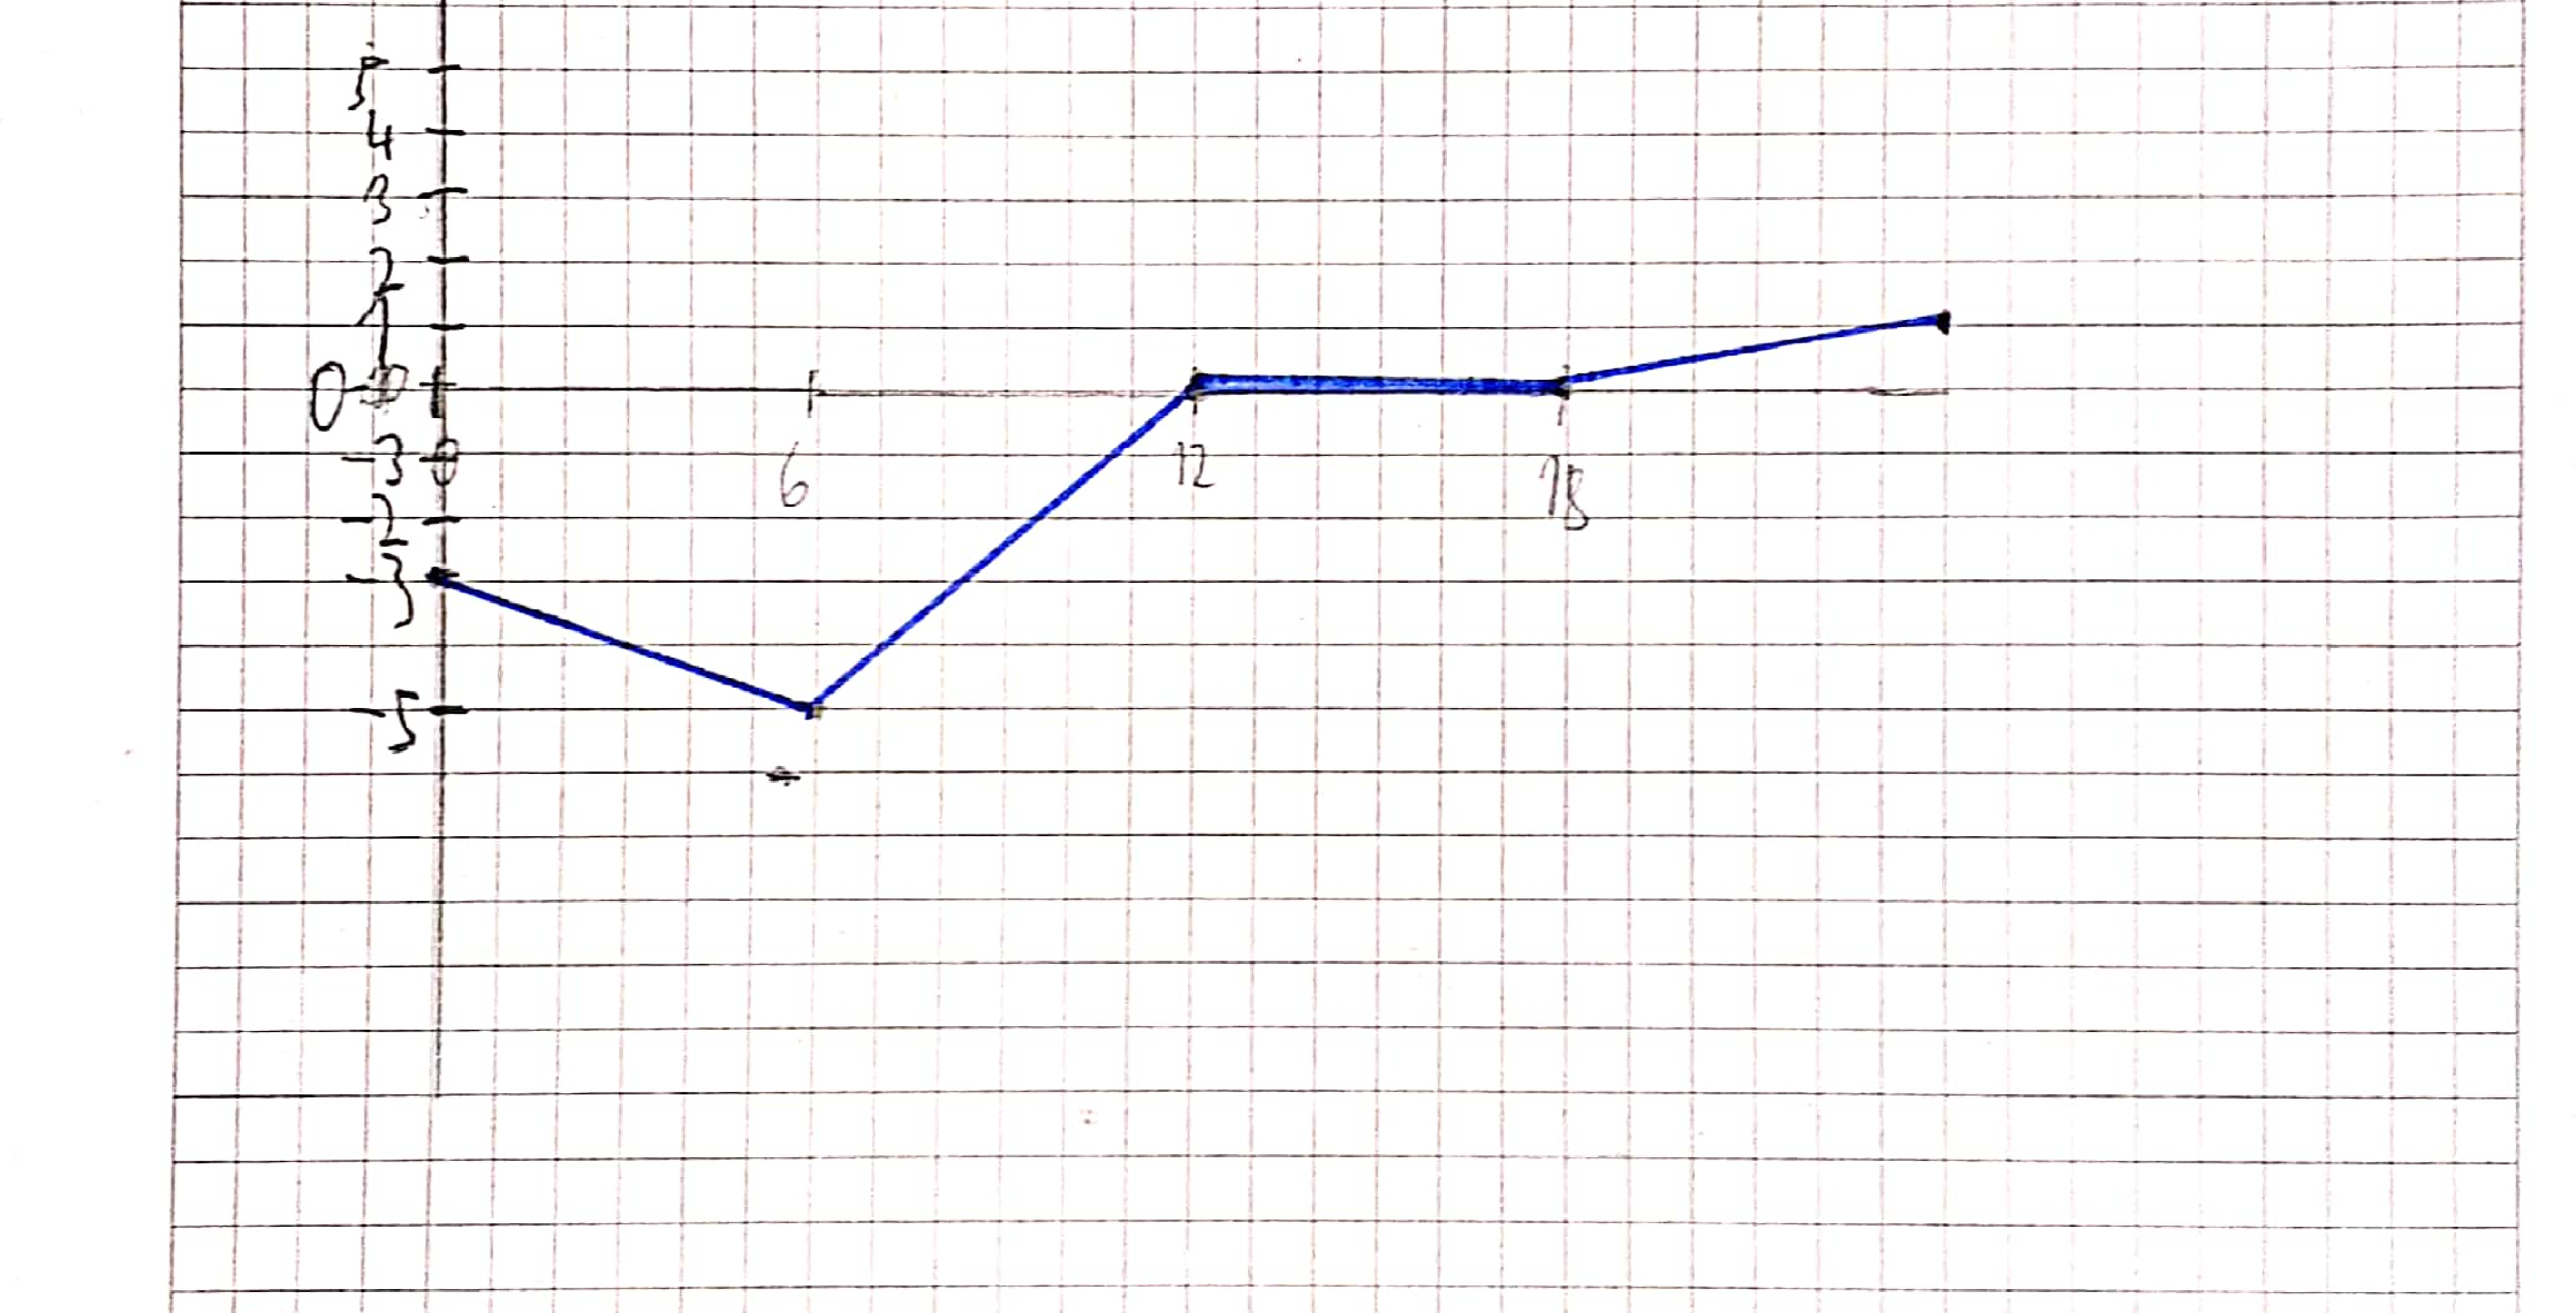
\includegraphics[scale=0.2]{./grafy/812/hand-812}
		\vskip 2cm
		\subsection{Priemery}
		\begin{tikzpicture}
		\begin{axis}[
			    title={Graf priemerných denných teplôt},
			    ylabel={$\overline{d_i}$},
			    xlabel={číslo dňa},
			    xmin=1, 
			    xmax=7,
			    ymin=-5, 
			    ymax=7,
			    xtick={1,2,3,4,5,6,7},
			    ytick={-5,0,5},
			    legend pos=north west,
			    ymajorgrids=true,
			    grid style=dashed,
		    ]		
		\addplot [
		    color=violet,
		    mark=*,
		]
		    coordinates {
			    (1,1)(2,0)(3,-2)(4,0.5)(5,-0.25)(6,0.5)(7,1.5)
		    };
		
	         \addlegendentry {Priemerná denná teplota od 6.12. do 12.12.}
		
		\addplot [
			color=red,
		]
			coordinates{
				(1,4)(7,4)
			};
			\addlegendentry {Najvyššia priemerná teplota v decembri v Bratislave}
			\addplot [
			color=blue,
		]
			coordinates{
				(1,-2)(7,-2)
			};
			\addlegendentry {Najnižšia priemerná teplota v decembri v Bratislave}
			\addplot [
			color=black,
		]
			coordinates{
				(1,1)(7,1)
			};
			\addlegendentry {Priemerná teplota v decembri v Bratislave}
			\addplot [
			color=black!30!green,
		]
			coordinates{
				(1,0.178)(7,0.178)
			};
			\addlegendentry {$\overline{t}$ -- priemerná týždenná teplota}



		\end{axis}
		\end{tikzpicture}
		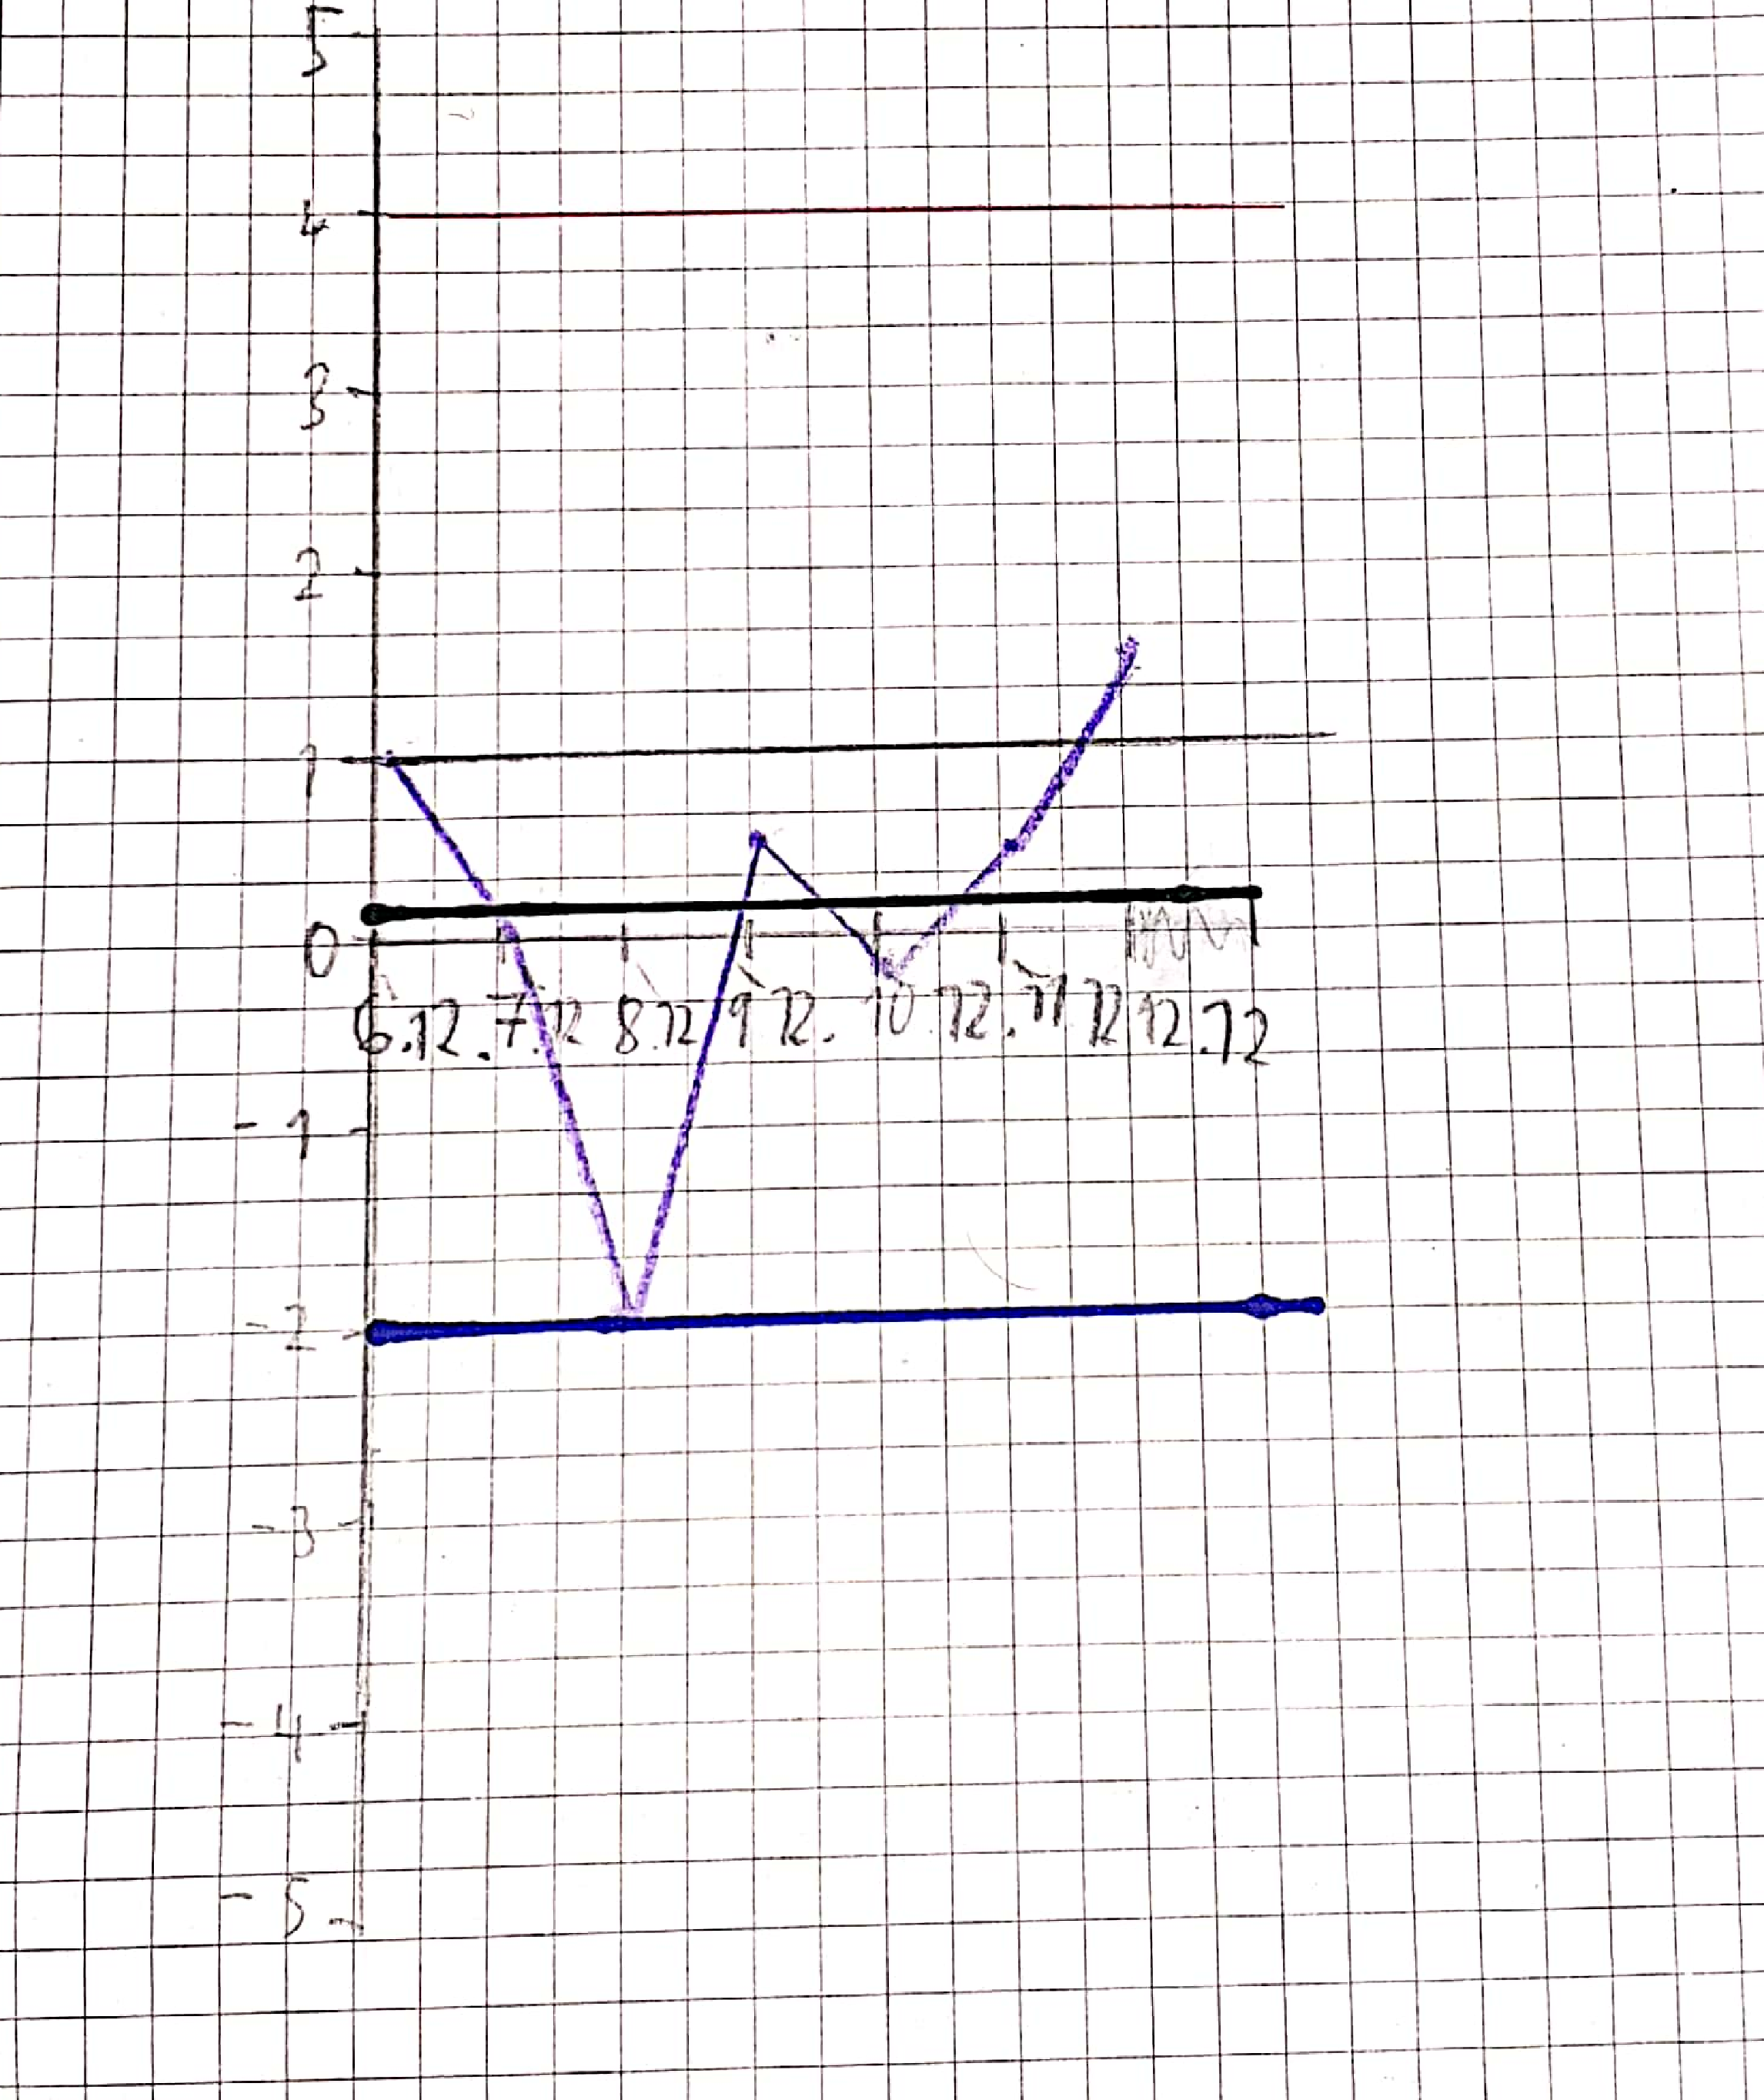
\includegraphics[scale=0.2]{grafy/priem/priem-hand}

	\end{center}
	\section{Záver}	
		Cieľom laboratórneho protokolu bolo meranie teploty v priebehu týždňa, počítanie týždenného priemeru teploty a porovnávanie tohto priemeru s priemernou teplotou v danom mesiaci v mieste merania.\\
		Vyšiel nám \textbf{týždenný priemer} $\overline{t} \approx \mathbf{0.178 °C}$\\
		Tento výsledok je relatívne k priemernej decembrovej teplote v mieste merania $\overline{p_t} = 1$ nízke a rozdiel týchto dvoch hodnôt $D_t = | \overline{p_t}-\overline{t}| = \mathbf{0.822 °C}$\\
		Najnižšia nameraná teplota $t_{min} = -5 °C$ bola nameraná ôsmeho decembra o šiestej hodine rannej.\\
		Najvyššia nameraná teplota $t_{max} = 3 °C $ bola nameraná siedmeho decembra o dvanástej hodine rannej.\\
		Najnižšia priemerná denná teplota $\overline{t}_{min} = -2 °C$ bola nameraná ôsmeho decembra.\\
		Najvyššia priemerná denná teplota $\overline{t}_{max} = 1.5 °C$ bola nameraná dvanásteho decembra.\\
		Poväčšine teplota počas dňa do dvanástej hodiny stúpala a potom klesala.\\
		Medzi výnimky patrí napríklad ôsmy december, kedy teplota do šiestej hodiny rannej klesala, potom vystúpila a na rovnakej teplote sa udržala až do šiestej hodiny večernej.\\
		Z \href{https://www.gtsforum.xyz/teploty}{interaktívneho grafu} ale aj z grafu priemernej dennej teploty vieme vyčítať, že do ôsmeho decembra teplota oscilovala a neskôr sa ustálila.\\
		$\overline{t}$ patrí do intervalu priemerných decembrových teplôt $\left(-2,4\right)$.\\
		Meranie mohlo ovplyvniť zaokrúhľovanie teplôt a to, že dáta neboli dátami v skutočnosti nameranými na mieste merania.
		Zlepšiť experiment by sa dalo používaním teplomerov.

		




	

\end{document}
